\documentclass{mcmthesis}
\mcmsetup{CTeX = false,   % 使用 CTeX 套装时,设置为 true
        tcn = 6666, problem = F,
        sheet = true, titleinsheet = true, keywordsinsheet = true,
        titlepage = true, abstract = true}
\usepackage{palatino}
\usepackage{lipsum}
\usepackage{hyperref}   %目录
\usepackage[UTF8, nocap]{ctex} %如果想使用中文输入的话,可以增加该宏包
\usepackage{indentfirst}  %首行缩进
\usepackage{booktabs}
\usepackage{tabularx}
\usepackage{amsmath}   %数学公式
\usepackage{xfrac}     %行间分式
\usepackage{latexsym}

\title{11.1   2020-F}
\author{pkx}

\date{\today}
\begin{document}

\begin{abstract}   %摘要

  \setlength{\baselineskip}{20pt}   %行间距20磅
\noindent 1. 这篇的一些笔记  \\
2. 尝试复现公式和表格  \\ 

\begin{keywords}
111; 222
\end{keywords}
\end{abstract}
\maketitle

\tableofcontents   %目录

\clearpage   %新开启一页

\section{NOTES}
\subsection{总的来说}

\indent\setlength{\parindent}{2em}
\setlength{\baselineskip}{20pt}   %行间距20磅
  整体结构框架跟第一篇大差不离,问题综述-背景介绍-问题分解-
  assumptions-models具体描述和policies制定-总结和sensitivity
   analysis  -strengthes and weakness. \\
\indent\setlength{\parindent}{2em}个别地方略有不同。

\begin{itemize}   %缩进
\item 第一篇先给出policies再进行models的描述,而这篇是根据models再给出politics design guided by the model,
      不过问题不是很大。可能写文章的时候要注意是否提及一下上面提到的policies。
\item 这篇把总结换了个说法 exhibition of results 并且放在了偏前面,第一篇把 conclusion 放在了最后,写的时候一些表述可能略有不同。没有给出improvements。
\item 感觉这篇的背景分析好像没有上一篇做的多?上一篇专门设置了一个部分
      Analysis of the Issue Paper
\end{itemize}

\subsection{一些有趣的地方}
\begin{itemize}
  \item 这篇 island country 的图很好看,貌似也有点难画orz。看起来很清晰明了,
        每个参数在立体图和展开图中一一对应。我读文章自己跟着算的时候也友好一些hhh
  \item 在EDP移民去向的问题上,这篇用了博弈论的方法,用大国之间政治力量施加压力来
        一次次进行迭代,最后得出满意的结果。而不是像上一篇单纯根据哪个国家应当承担
        的责任比较重来进行分配。这个角度感觉蛮有意思的,我觉得可以两者结合一下试试看。\\
        博弈论这块没有怎么太了解过,一路跟着看下来有点懵……
  \item 
\end{itemize}

\subsection{迷惑}
\begin{enumerate}
  \item 感觉这篇笔误有点多,不知道是原文就这样还是资源有小问题?
  \item table2 到table3 的变化,原因只说了 countries will do sth,具体是怎么
        变化为什么的好像没有说的太明白,是不是应该给数据什么的?
  \item 不太明白5.3.2 Game rules 这里,$FH^+ = [fh^{+}_{ij}]_{8\times i}$ 
        这个式子是怎么得出来的
  \item 6.2彻底懵圈
\end{enumerate}

\subsection{一些句子}
\begin{enumerate}[(1)]
  \item Research has identified a fact that several are at risk of xxx. 
  \item This put the problem of xxx forward for the international society.
  \item According to the research conducted by the former people, we get to know。。。
  \item with reasonable inference
  \item Up to now we have illustrated three things:
  \item Now we’ll research the sensitivity of the two parameters to perfect our
  discussion.
\end{enumerate}
  
\section{公式和表格}

\subsection{表格}
\begin{table}[htbp] 
  \setlength{\abovecaptionskip}{-10pt}   %调整标题与表格的间距
  \setlength{\belowcaptionskip}{10pt}
  \centering
	\caption{\label{tab:test}Declaration}  %标题
		\begin{tabular}{ccl} %三列,居左,中,左
 		\toprule %第一条线
     Symbols & Unit & Description of notations and signs \\ 
  	\midrule %第二条线
 		$v$ & $m \cdot a^{-1} $ & The speed of raising sea level \\ 
 		$P_t$ & - &  the international pressure \\ 
  \bottomrule %第三条线
 \end{tabular} 
\end{table}

\begin{table}[htbp] 
  \setlength{\abovecaptionskip}{-0pt}   %调整标题与表格的间距
  \setlength{\belowcaptionskip}{10pt}
  \centering
	\caption{\label{tab:test}World-Constant condition}  %标题
		\begin{tabular}{cccc} 
 		\toprule %第一条线
     Years(since 2020) & Raised Sea Level(m) & Sink territory(km$^2$) & influenced people \\ 
  	\midrule %第二条线
 		2050 & 0.11 & 45,303/0.04\%  & 19,046,347/0.22\% \\ 
    2100 & 0.304 & 120,787/0.11\% & 50,781,761/0.59\% \\ 
    2170 & 0.57 & 226,425/0.20\% & 95,172,506/1.11\% \\
    2220 & 0.76 & 301,851/0.26\% & 126,855,452/1.48\% \\
  \bottomrule %第三条线
 \end{tabular} 
\end{table}

\begin{table}[htbp] 
  \setlength{\abovecaptionskip}{-0pt}   %调整标题与表格的间距
  \setlength{\belowcaptionskip}{10pt}
  \centering
	\caption{\label{tab:test}Ranks of Countries Responsibility}  %标题
		\begin{tabular}{cc|cc} 
 		\toprule %第一条线
     Country & $R_{country}$ & Country & $R_{country}$ \\ 
  	\midrule %第二条线
 		US & 0.991 & Canada & 0.276 \\ 
    China & 0.671 & French & 0.258 \\ 
    Japan & 0.316 & Brazil & 0.256 \\
    Russian & 0.300 & Australia & 0.249 \\
  \bottomrule %第三条线
 \end{tabular} 
\end{table}

\subsection{公式}

$\begin{cases}x+y>1-x-y\\x+1-x-y>y\\y+1-x-y\end{cases}$

\begin{equation}
  %\label{eq6}
  \left\{
  \begin{aligned}   % &的位置就是对齐的位置
  &R=\sqrt{\dfrac{-H^2+\sqrt{H^4+\dfrac{4S^2}{\pi^2}}}{2}} \\ 
  &L=\dfrac{S}{\pi}\sqrt{\dfrac{2}{-H^2+\sqrt{H^4+\dfrac{4S^2}{\Pi^2}}}}\\
  &A=\dfrac{R}{L}
  \end{aligned}
  \right.
\end{equation}

\begin{equation}
  \int_0^L A\cdot 2\pi lpdl = \int_0^L Ak\cdot 2\pi l^2 dl 
  =P_A \Rightarrow k=\dfrac{3P_A}{2A\pi L^3}
\end{equation}

\begin{equation}
  a=\dfrac{v_{2014}-v_{2002}}{2014-2002} = 0.0925 mm\cdot a^{-2} \approx 0.01 mm\cdot a^{-1}
\end{equation}

\begin{equation}
  x_i=(x_{i1},x_{i2}) \in \{(0,0),(0,1),(1,0),(1,1)\}
\end{equation}

\begin{equation}
  x_i =(0,0) \to x_i =(0,1)
\end{equation}

\begin{equation}
  X=(x_1,x_2,…,x_8)=
  \begin{bmatrix}
    x_{11} & x_{21} &\dots &x_{81}\\
    x_{12} & x_{22} &\dots &x_{82}\\
  \end{bmatrix}
\end{equation}

\begin{equation}
  \left\{
  \begin{aligned}   % &的位置就是对齐的位置
  &\dfrac{\partial S}{\partial V_0} = \dfrac{\pi L^2}{H^2} (\dfrac{2H}{y}-2v_0-ay)\\ 
  &\dfrac{\partial ^2 S}{\partial v_0^2}=-\dfrac{2\pi L^2}{h^2}\\
  \end{aligned}
  \right.
\end{equation}

\begin{equation}
  \triangle_f = c^2 - 4ab = \dfrac{4k_b^2 (k_b(p+p\alpha)-2k_d)(k_b(p-p\alpha)+2k_d) }{(k_b p\alpha - 2k_d)^2}
\end{equation}

\emph{center of percussion} [Brody 1986]

\begin{Theorem}    %定理
\label{thm:latex}
\LaTeX
\end{Theorem}
\begin{Lemma} 
\label{thm:tex}
\TeX .
\end{Lemma}
\begin{proof}
The proof of theorem. \footnote{这是一个脚注}   %脚注
\end{proof}

\section{Analysis of the Problem}
\begin{figure}[h]
\small
\centering
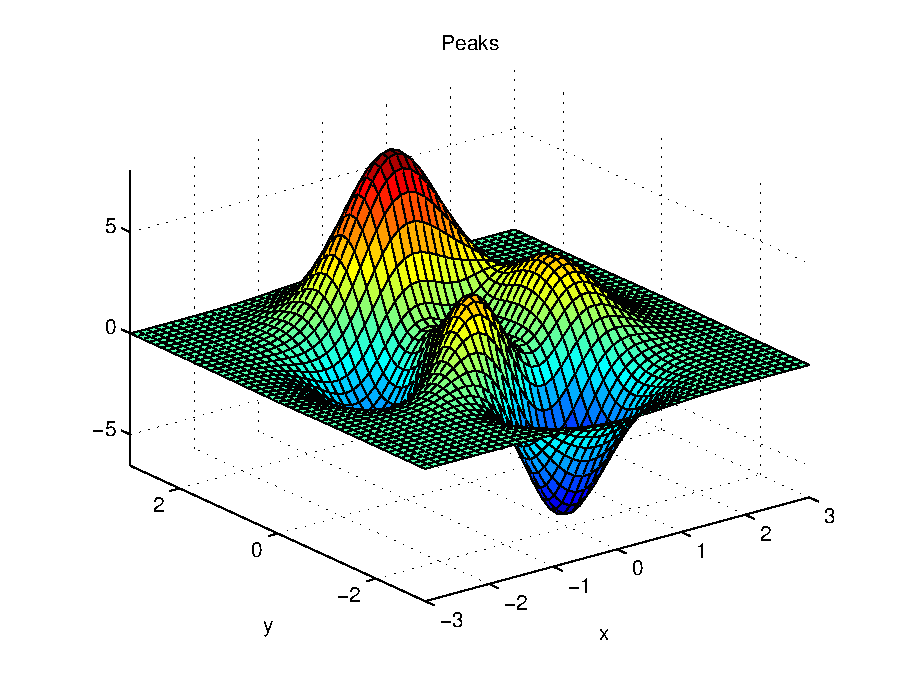
\includegraphics[width=12cm]{mcmthesis-aaa.eps}
\caption{aa} \label{fig:aa}
\end{figure}

\eqref{aa}
\begin{equation}
a^2 \label{aa}
\end{equation}

\[
  \begin{pmatrix}{*{20}c}
  {a_{11} } & {a_{12} } & {a_{13} }  \\
  {a_{21} } & {a_{22} } & {a_{23} }  \\
  {a_{31} } & {a_{32} } & {a_{33} }  \\
  \end{pmatrix}
  = \frac{{Opposite}}{{Hypotenuse}}\cos ^{ - 1} \theta \arcsin \theta
\]

\[
  p_{j}=\begin{cases} 0,&\text{if $j$ is odd}\\
  r!\,(-1)^{j/2},&\text{if $j$ is even}
  \end{cases}
\]

\[
  \arcsin \theta  =
  \mathop{{\int\!\!\!\!\!\int\!\!\!\!\!\int}\mkern-31.2mu  
  \bigodot}\limits_\varphi
  {\mathop {\lim }\limits_{x \to \infty } \frac{{n!}}{{r!\left( {n - r}
  \right)!}}}   \eqno[1] 
\]
减号 “-” 后面的数字可以自己根据情况调整,数值越大,斜杆越往字母左侧移动

\section{Calculating and Simplifying the Model  }

\section{The Model Results}

\section{Validating the Model}

\section{Conclusions}

\section{A Summary}

\section{Evaluate of the Mode}

\section{Strengths and weaknesses}


\subsection{Strengths}
\begin{itemize}
\item \textbf{Applies widely}\\
This system can be used for many types of airplanes.
\item \textbf{Improve the quality of the airport service}\\
Balancing the cost of the cost and the benefit. 
\end{itemize}

\begin{thebibliography}{99}
\bibitem{1} D.~E. KNUTH   The \TeX{}book  the American
Mathematical Society and Addison-Wesley
Publishing Company , 1984-1986.
\bibitem{2}Lamport, Leslie,  \LaTeX{}: `` A Document Preparation System '',
Addison-Wesley Publishing Company, 1986.
\bibitem{3}\url{http://www.latexstudio.net/}
\bibitem{4}\url{http://www.chinatex.org/}
\end{thebibliography}

\begin{appendices}

\section{First appendix}

aaaaa

Here are simulation programmes we used in our model as follow.\\

\textbf{\textcolor[rgb]{0.98,0.00,0.00}{Input matlab source:}}
\lstinputlisting[language=Matlab]{./code/mcmthesis-matlab1.m}

\section{Second appendix}

some more text \textcolor[rgb]{0.98,0.00,0.00}{\textbf{Input C++ source:}}
\lstinputlisting[language=C++]{./code/mcmthesis-sudoku.cpp}

\end{appendices}
\end{document}

%% 
%% This work consists of these files mcmthesis.dtx,
%%                                   figures/ and
%%                                   code/,
%% and the derived files             mcmthesis.cls,
%%                                   mcmthesis-demo.tex,
%%                                   README,
%%                                   LICENSE,
%%                                   mcmthesis.pdf and
%%                                   mcmthesis-demo.pdf.
%%
%% End of file `mcmthesis-demo.tex'.
